\chapter{Path Indexing}
In this section we give an informal overview of path indexing and take a closer look at some details of its implementation in Isabelle/ML.\\
\section{Theory}
A path index is used to store a collection of terms for efficient querying. The queries commonly include retrieval of generalisations or unifiables of a term from the collection.\\
The core concept on which path indexing is based is the mapping of each symbol in a term to a path. This path consists of the nodes traversed from the root to the symbol. In the standard tree form this is an alternating sequence of symbols and the index of the argument which is traversed next. Additionally this path starts with the root symbol and ends with the symbol being addressed. As a result a single term is described by a collection of paths. We ignore the identity of variables as they are mostly irrelevant for the queries and increase memory consumption.\todo{update graphic accordingly. Move somewhere else}\\
\begin{figure}[h]
\centering
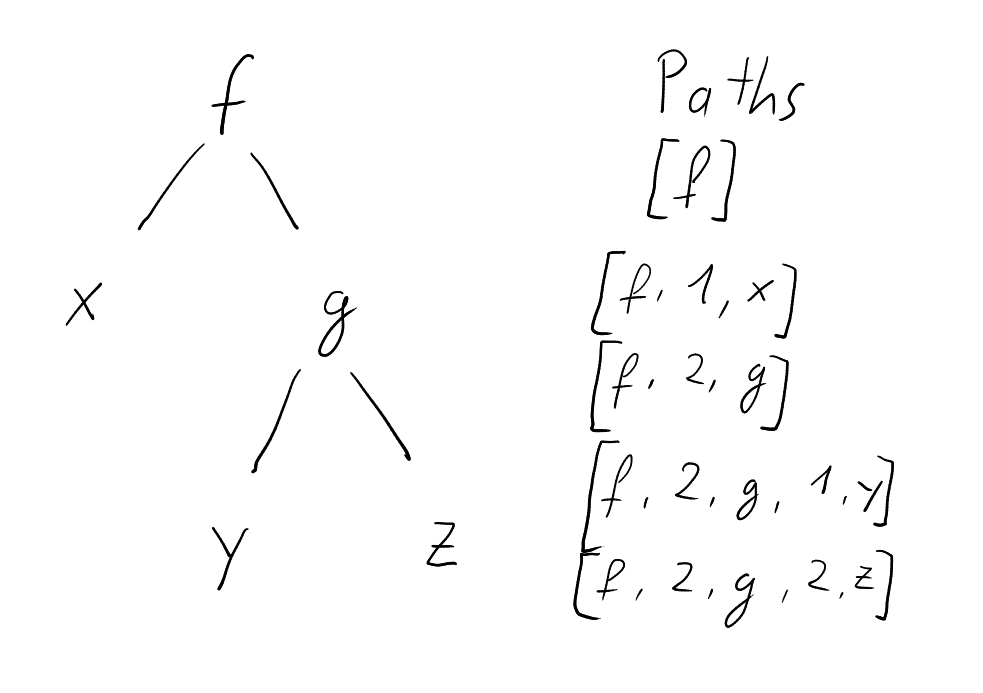
\includegraphics[scale=0.25]{figures/term_path.png}
\caption{A term and the paths associated with its symbols}
\end{figure}\\
To store the paths of different terms within one index we must associate each path with a list of terms within which this path occurs. These are called path lists. As a term is described by a path for each symbol each term is generally saved in many path lists.\\
For storage of the paths we chose a trie-based approach. This reduces the memory required as the paths of a term often share prefixes. Furthermore inserting a term similar to one already present profits from the same sharing of prefixes.\\
The queries are based on intersections and unions of the different path lists to enforce constraints on the terms. The simplest query is the lookup of identical terms, for example to check if a term is already contained within the index. To answer the query we first build a list of the paths the term contains. Next we lookup the path lists corresponding to them in the index. The intersection of these path lists returns all terms containing symbols at identical paths as the query term. Under the assumption of type correctness\todo{lookup correct term} across terms only the original or no term is retrieved.\\
To retrieve the unifiables of a term from the index we can use some observation on the unification problem.
\begin{enumerate}
  \item A variable is unifiable with any other term
  \item Every other symbol\todo{Name for ``every other symbol/terminal''? Fixed vars? Constants?} is unifiable with itself and variables
  \item A function $f(x_{1},...,x_{n})$ is unifiable with term $t$ if $t$ is a variable or the function symbols of $f$ and $t$ are identical and $x_{1},...,x_{n}$ are unifiable with the respective argument of $t$
\end{enumerate}
Using this we can define an algorithm recursing on the structure of the query term while intersecting and unifying the different path lists of the index. The different query types share parts with the lookup being the most restrictive and the unifiables the least restrictive.\\
We use the syntax $<p \cdot 1 \cdot a>$ to describe the path reached by traversing the first argument of $p$ which must be an $a$. $PathList(p)$ refers to the path list stored at the path $p$. $AllTerms$ is the collection of all terms stored in the index.
\begin{figure}[h]
\centering
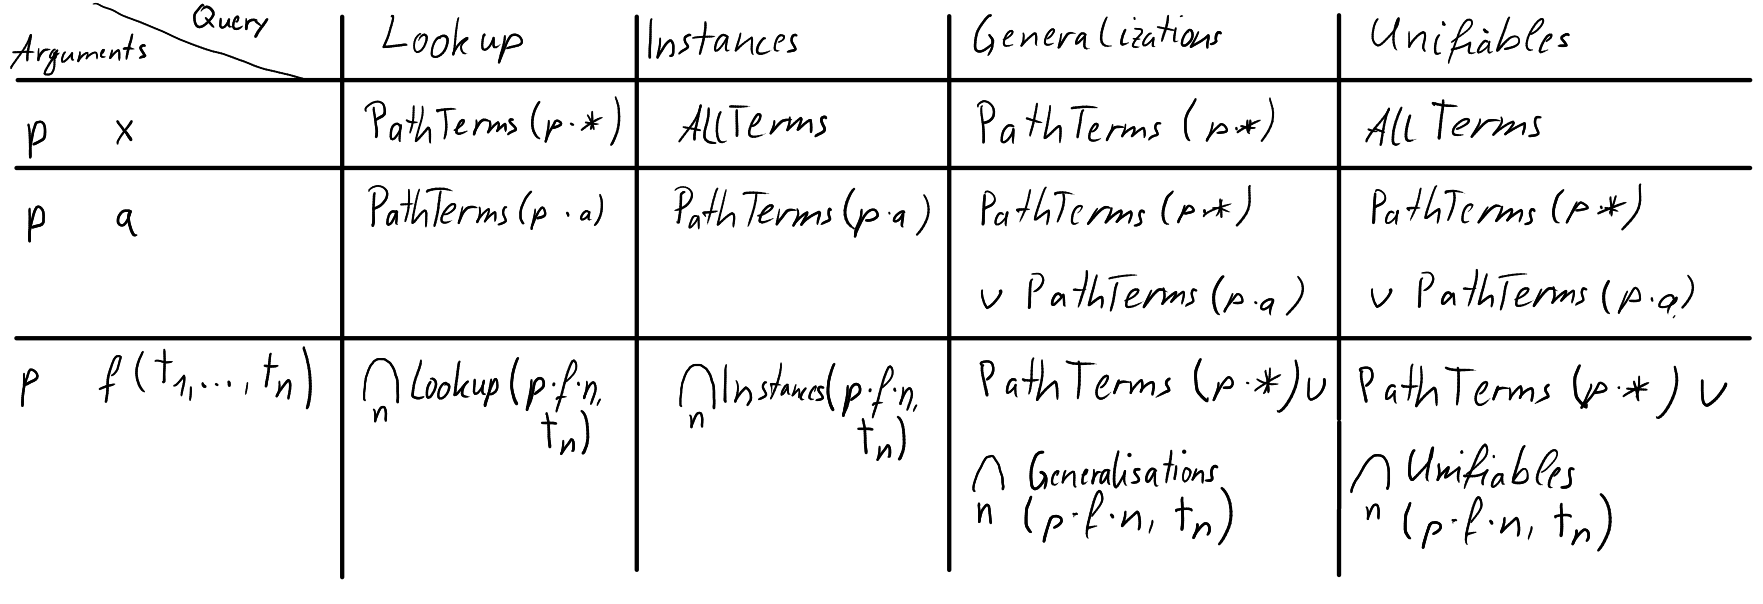
\includegraphics[scale=0.25]{figures/queries.png}
\caption{The different queries and their definition}
\end{figure}\\
We can see in the table that the different queries share many similarities with the $Unifiables$ being a combination of $Instances$ and $Generalizations$.

\section{Implementation in Isabelle/ML}
The efficient implementation of path indexing relies on a number of optimizations. Data Sharing in Poly/ML. Intersect at end for cache. Efficient intersect with OrdList. pointereq. Saving values separately. NoConstraint exc.
